\documentclass[a4paper,11pt]{article}
\usepackage[a4paper]{geometry}
\geometry{hmargin=2cm, vmargin=1.7cm}
\usepackage{hyperref}
\usepackage{fontspec}
\usepackage{xunicode}
\usepackage{xltxtra}
%\setmainfont{Linux Libertine}
\setsansfont{DejaVu Sans}
\usepackage{polyglossia}
\setdefaultlanguage{french}
\usepackage{minted}
\usepackage{algorithm}
\usepackage{algorithmic}
%\usepackage{titlesec}
\usepackage{amsmath}
\usepackage{subcaption}
%\titleformat*{\section}{\large\bfseries\sffamily}
%\titleformat*{\subsection}{\bfseries\sffamily}

\title{Théorie des graphes \\ --- \\ Rapport}
\author{Élie \textsc{Bouttier} \\ Franklin \textsc{Delehelle}}
\date\today

\begin{document}

\maketitle


% Page de présentation
%\begin{center}
%\thispagestyle{empty}
%~\\
%\vspace{5cm}
%{\Huge \sffamily Rapport de théorie des graphes}\\
%\vspace{5cm}
%Élie \textsc{Bouttier} \& Franklin \textsc{Delehelle}\\
%\end{center}
%\newpage



% Début effectif du document
%\section{Introduction}
\begin{abstract}
Nous avons décidé d'utiliser l'opportunité qui nous était offerte de travailler
sur ce projet pour implémenter 
un algorithme de \emph{pathfinding} pour un robot qui participera à la coupe de
France de robotique 2013.
\end{abstract}

\section{L'algorithme}
Nous avons choisi d'utiliser JPS\footnote{Jump Point Search}, un algorithme très
récent, puisque publié en
2011\footnote{\url{http://grastien.net/ban/articles/hg-aaai11.pdf}}, qui permet
d'optimiser l'algorithme bien connu d'A* en ne le 
développant que là où nécessaire ; pour cela, il utilise deux règles :
\begin{description}
\item[règle d'élagage] pour tout point $x$ atteint depuis $p$, on supprime tout
    ses voisins $n$ dont soit le chemin $(p,y,n)$
    ou $(p,n)$ est plus court que $(p,x,n)$, ou bien dont les chemins $(p,y,n)$
    et $(p,x,n)$ ont la même longueur, mais dont le
    chemin $(p,y,n)$ comporte un mouvement diagonal plus tôt que $(p,x,n)$. Les
    voisins conservé après cet élagage sont appelés 
    \emph{voisins naturels} de $x$. Les voisin supplémentaires entre les cas où
    $x$ est entouré de vide et le voisinage de $x$ 
    contient un obstacle sont appelés \emph{voisins forcés}.

\item[règle de saut] les sauts consistent, plutôt que de considérer le voisin
    immédiat, à évoluer dans une direction donné jusqu'à trouvé un nœud
    possédant des \emph{voisins forcés}. Un tel nœud est appelé \emph{jump
    point}.
\begin{figure}[h]
\centering
\begin{subfigure}{.3\textwidth}
\centering
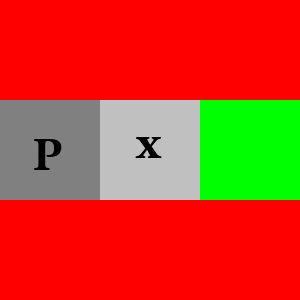
\includegraphics[width=0.5\linewidth]{droit.png}
\caption{Élagage horizontal}
\end{subfigure}
\begin{subfigure}{.3\textwidth}
\centering
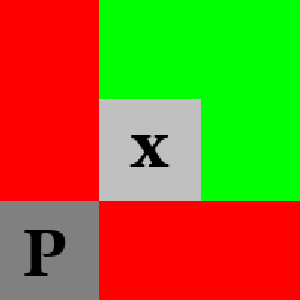
\includegraphics[width=0.5\linewidth]{diag.png}
\caption{Élagage diagonal}
\end{subfigure}
\begin{subfigure}{.3\textwidth}
\centering
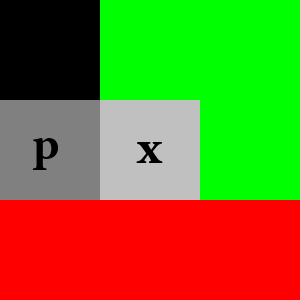
\includegraphics[width=0.5\linewidth]{obstacle.png}
\caption{Cas d'un obstacle}
\end{subfigure}
\caption{En rouge, les voisins éliminés, en vert, les voisins à explorer, en 
noir, les obstacles, en gris clair, le point courant et en gris foncé le point d'origine}
\end{figure}

Dans le cas où l'exploration dans la direction courante est arrêtée par un
obstacle, le chemin y menant depuis le dernier 
changement de direction est purement oublié.

Toutefois, la direction courante est privilégiée, et les voisin induisant un
changement de direction ne sont explorés que si
la poursuite de l'exploration de la direction courante échoue.
\end{description}

Enfin, l'algorithme A* est appliqué à chacun des nœuds marqués par JPS jusqu'à
trouver le point cible, qui est alors relié au 
nœud qui a permis de le trouver. Précisons que l'algorithme fonctionne en une
seule étape : il ne s’agit pas de déterminer les \emph{jump points} puis
d’utiliser l'algorithme A*, les \emph{jump points} sont déterminés au fur et à
mesure de l’exploration par l'algorithme A*.

\section{Performances}
Le nombre de nœuds développé en utilisant l'algorithme JPS se trouve
de toute évidence considérablement réduit. Ceci est encore plus vrai si la zone
à explorer possède peu d’obstacle.

L’utilisation de l’algorithme A* est dans certain cas tellement lente qu’on
procède à une première étape de squelettisation afin de lancer l’algorithme sur
un graphe de moins grande envergure. Bien que l’utilisation de l’A* sur ce
nouveau graphe se trouve être plus rapide que l’utilisation du JPS sur
l’ancien, ce dernier se trouve dans la grande majorité des cas être globalement
plus rapide car ne nécessitant pas de pré-traitement.

Bien que présentant globalement de meilleures performances, l'utilisation de
l'algorithme JPS pose des contraintes sur le déplacement, puisqu'il requiert
absolument la possibilité du déplacement en diagonal et l'utilisation de la
distance quadratique comme heuristique. Soulignons tout de même
que l'algorithme propose une solution optimale !

\section{Implémentation}
Nous avons décidé d'implémenter le cœur de l'algorithme sous la forme d’une
bibliothèque partagée, codée en C afin de bénéficier
au mieux de la rapidité du code natif.

Toutefois, dans le but de simplifier son utilisation et son interfaçage avec des
programmes de test, nous avons écrit un 
\emph{wrapper} python qui nous permet de profiter de la vitesse de l'algorithme
implémenté en C avec la facilité de développement 
et de debuggage d'un langage haut niveau comme python.

C'est ainsi que nous avons pu développer rapidement et simplement les programmes
de démonstration inclus dans notre projet.

\vspace{0.2cm}
\begin{center}
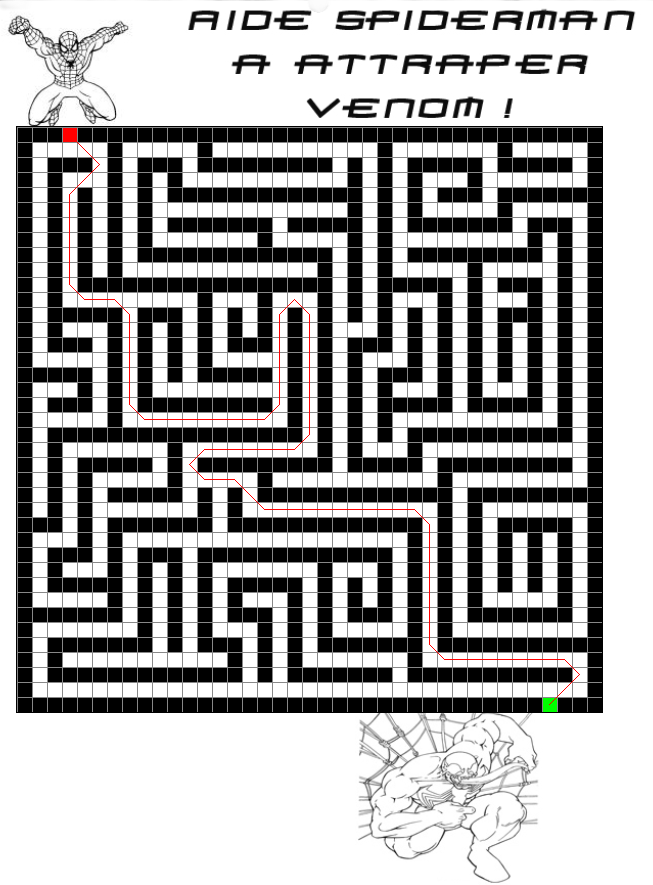
\includegraphics[width=0.5\linewidth]{screenshot/spiderman.png}
\end{center}

\end{document}
